\documentclass[a4paper, 12pt, oneside]{article}
\usepackage{graphicx}
\begin{document}

\begin{titlepage} % Suppresses headers and footers on the title page

	\centering % Centre everything on the title page
	
	\scshape % Use small caps for all text on the title page
	
	\vspace*{\baselineskip} % White space at the top of the page
	
	%------------------------------------------------
	%	Title
	%------------------------------------------------
	
	\rule{\textwidth}{1.6pt}\vspace*{-\baselineskip}\vspace*{2pt} % Thick horizontal rule
	\rule{\textwidth}{0.4pt} % Thin horizontal rule
	
	\vspace{0.75\baselineskip} % Whitespace above the title
	
	{\LARGE Consultant Tracker\\Architectural Design} % Title
	
	\vspace{0.75\baselineskip} % Whitespace below the title
	
	\rule{\textwidth}{0.4pt}\vspace*{-\baselineskip}\vspace{3.2pt} % Thin horizontal rule
	\rule{\textwidth}{1.6pt} % Thick horizontal rule
	
	\vspace{2\baselineskip} % Whitespace after the title block
	
	
	%------------------------------------------------
	%	Editor(s)
	%------------------------------------------------
	
	Edited By
	
	\vspace{0.5\baselineskip} % Whitespace before the editors
	
	{\scshape\Large Sibekezelo Mamba 16095414 \\ Johan de Waal 16155140 \\ Stephen Munro 16024479\\ Hulisani Mudimeli 			16073364 \\ Ngonidzashe Mujuru 16285256  \\ Tatenda Mafunga 16094965\\} % Editor list
	
	\vspace{0.5\baselineskip} % Whitespace below the editor list
	
	\textit{University of Pretoria \\2018} % Editor affiliation
	
	\vfill % Whitespace between editor names and publisher logo
	
\end{titlepage}

\newpage
\tableofcontents
\newpage


\pagenumbering{arabic}

\section{Introduction}

\subsection{Purpose}
	The purpose of this document is to provide a high level overview of the Consultant Tracker system. The document will illustrate and explain the architectural design of the system, the use cases supported by the system and architectural styles and components that have been selected. 

\subsection{Overwiew}
	This document will begin by giving an overall description of the system. This will include the the architecture style and design chosen for the system and a deployment diagram used for diagramatic representation of the system as a whole.
\newpage
\section{Overall Description}

\subsection{Architectural Style}
	The system has been identified to be an interactive system. It will be deployed as a hybrid system which is composed of a model-view-controller architecture and a three-tier architecture.The architecture will be split into three distinct layers:
\begin{enumerate}
	\item Presentation Layer
		\\This will be responsible for displaying data in a particular format.
	\item Logic Layer
		\\ This layer will work hand in hand with the controller. The controller will be reponsible for data processing, as well as the extraction and insertion of data to and from the data layer. This layer will ensure that all business rules are satisfied.
	\item Data Layer
		\\This is responsible for storage of project data and consultant data.
\end{enumerate}

\newpage
\subsection{Architecture Summary}
A breakdown of the system and the various technologies used is shown below.
\newline
\begin{figure}[h!]
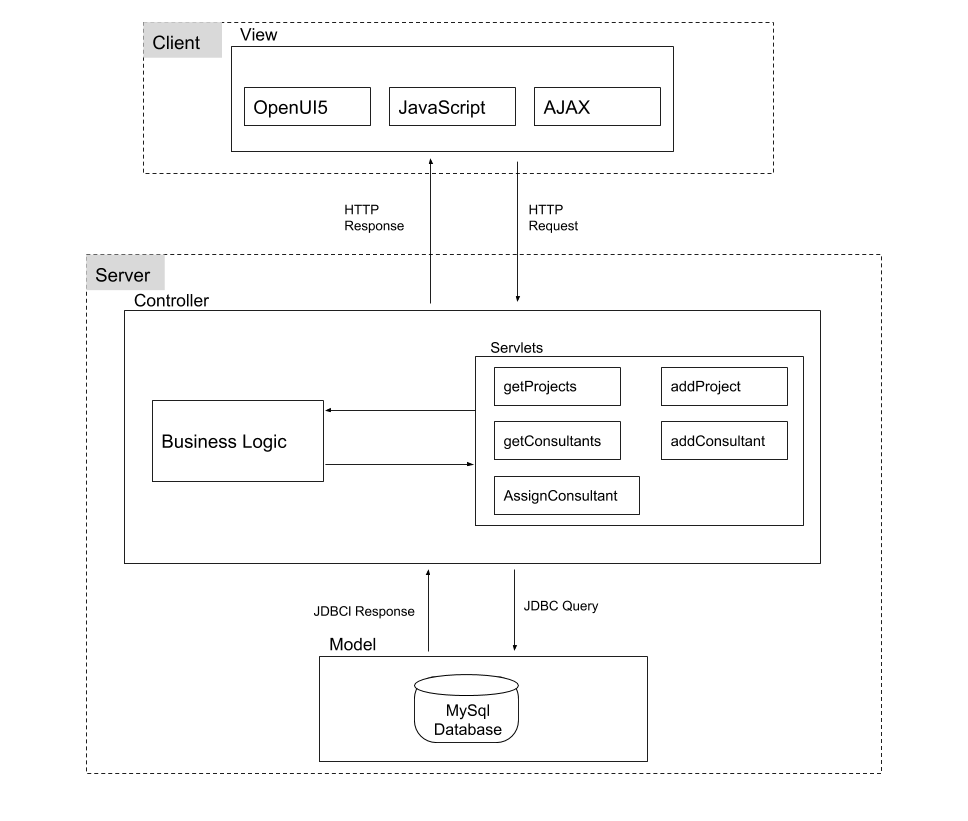
\includegraphics[width = \linewidth]{images/summary.png}
	\caption{System breakdown}
\end{figure}
\newline
Technologies used include:
\begin{itemize}
	\item Layer 1 - View
	\begin{itemize}
		\item OpenUI5
		\item JavaScript
		\item AJAX
	\end{itemize}
	\item Layer 2 - Controller
	\begin{itemize}
		\item Java
		\item Java Persistence API
	\end{itemize}
	\item Layer 3 - Model 
	\begin{itemize}
		\item MySQL
		\item JDBC Sql Connector
	\end{itemize}
\end{itemize}

\section{User Roles}
The system will consist of two users, namely an administrator and a consultant. Their roles are outlined below.
\begin{itemize}
\item Administrator
\begin{itemize}
\item Login
\item CRUD Projects
\item CRUD consultants
\item Assign/remove consultants from a project
\item Communicate with consultants.
\item View projects currently running
\end{itemize}
\item Consultant
\begin{itemize}
\item Login
\item View assigned projects
\item Communicate with administrator
\end{itemize}
\end{itemize}

\section{Quality Requirements}
\subsection{Security}
The system will make use of two methods to achieve security.This will include:
\begin{itemize}
\item role based management
\item user authentication
\end{itemize}
\subsection{Usability}
\begin{itemize}
	\item The system must be easy to learn.
	\item The user interface must be easy to use and must be intuitive.
	\item The system should display options in a logical manner.
	\item Incorporate widgets and icons that the target users may be familiar with.
	\item The user manual should have a detailed description of the system.
\end{itemize}

\section{Deployment Diagram}
	The system structure is depicted in the deployment diagram below.
\newline
\begin{figure}[h!]
	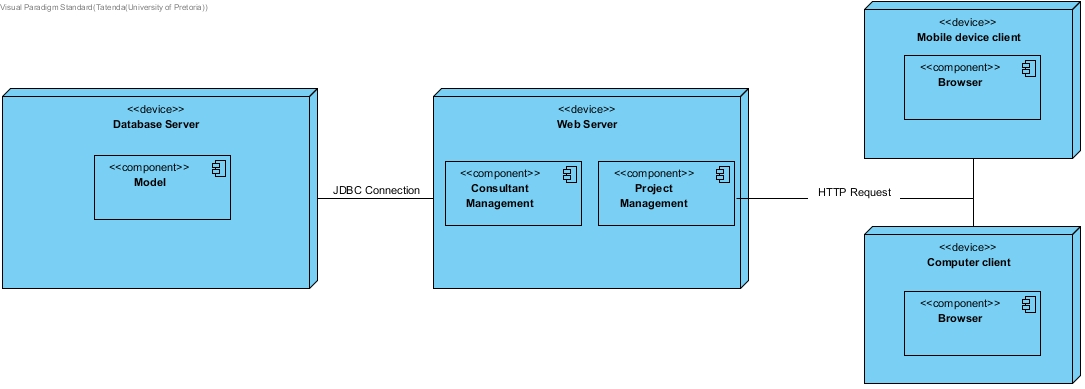
\includegraphics[width=\linewidth]{images/deployment.png}
	\caption{Deployment diagram}
\end{figure}
\end{document}
